\documentclass[conference]{IEEEtran}
\IEEEoverridecommandlockouts
% The preceding line is only needed to identify funding in the first footnote. If that is unneeded, please comment it out.
\usepackage{cite}
\usepackage{tabularx}
\usepackage{amsmath,amssymb,amsfonts}
\usepackage{algorithmic}
\usepackage{graphicx}
\usepackage{textcomp}
\usepackage{xcolor}
\def\BibTeX{{\rm B\kern-.05em{\sc i\kern-.025em b}\kern-.08em
    T\kern-.1667em\lower.7ex\hbox{E}\kern-.125emX}}
\begin{document}


\title{%
  Directional Stock Prediction Using Viral Tweets and News References 
\\[.3in]
  \large Project Proposal \\
CSE 573 - Spring 2022 \\ 
Arizona State University \\
}


\author{\IEEEauthorblockN{Hadi Mazboudi}
    \IEEEauthorblockA{hmazboud@asu.edu}
    \IEEEauthorblockA{SCAI}
    \and
    \IEEEauthorblockN{Brian Nguyen}
    \IEEEauthorblockA{bnguye23@asu.edu}
    \IEEEauthorblockA{SCAI}
    \and
    \IEEEauthorblockN{Joseph Dicke}
    \IEEEauthorblockA{jdicke@asu.edu}
    \IEEEauthorblockA{SCAI}
    \and
    \IEEEauthorblockN{Crystal Nguyen}
    \IEEEauthorblockA{cnguye30@asu.edu}
    \IEEEauthorblockA{SCAI}
    \and
    \IEEEauthorblockN{Rushil Popat}
    \IEEEauthorblockA{rushil@asu.edu}
    \IEEEauthorblockA{SCAI}

}




\maketitle

\begin{abstract}
    There is an incredible financial incentive to “solving” the problem of optimizing trading in the stock market. Many ideas have been tried and tested to varying degrees of success, basing their trading strategies on either mathematical models of ideas of momentum of the stock, volume, or other technical indicators. In this paper, we will discuss the development of several different trading strategies using modern machine learning and natural language processing. In this experiment, we will be applying our methodologies to the stocks of Amazon.com, Inc. (AMZN) and Apple Inc. (AAPL). Our data set includes over 100,000 news articles and tweets related to these tickers and market data for both stocks at the closing time between November 2017 and February 2019, which is the time interval we will be using to develop our trading strategies. In this paper, we will discuss the development of our strategies, which will be a combination of word encoders (Word2Vec, BERT, and Topic Modeling), sentiment analysis, and machine learning models (logistic regression). In this paper, we will outline our research plan, evaluation metrics, and timeline for the completion of the experiment.
\end{abstract}

\begin{IEEEkeywords}
    Natural language processing, BERT, Word2Vec, Topic Modeling, classification, Tweets, stocks
\end{IEEEkeywords}

\section{Introduction}
The stock market allows people to purchase a public company’s stock, which is a small piece of that company \cite{b2}. The price of a stock can be affected by a number of different factors such as changes within the overall economy, changes within the industry, political events, war, decisions by company executives, environmental changes, and changes in customer behavior. Oftentimes, people purchase stocks in order to invest their money rather than putting their money in a savings account at a bank due to the higher potential growth rates.

Lately, the United States has seen that news articles and social media, particularly tweets from the popular micro-blogging platform Twitter, have begun to have an effect on stock prices. Most companies have an online social media presence on platforms such as Twitter and people that invest in these companies can infer stock price information from the sentiment and subject matter of the tweets coming from companies or accounts which have access to company information \cite{b6}. A notable example is when Elon Musk tweeted about thinking about taking his company Tesla, Inc. (TSLA) private at \$420 after he had secured funding. After this tweet, the stock price increased dramatically \cite{b4}.

It is nearly impossible for one single person to keep up with the constant bombardment of information coming out on news articles and Twitter, so our idea was to use this plentiful information and build models that can help predict stock price movement based on this information. We used textual information by performing Natural Language Processing techniques like BERT and sentiment analysis on the data sets soon to be described and used them to train our stock prediction models.

\section{Problem Statement}
The goal of this project is to feed a tweet's URL into our system, which will then parse the tweet and feed the text into the three models that we have created. After the result is generated it is sent to our HTML interface and will display either an up or down arrow for what each model calculated. From the three results the majority of up or down arrows determine a larger up or down arrow that is displayed to tell the user which direction the models believe the stock will go. The problem that we are tackling is the issue with tweets having an effect on stock price. We can often observe that stocks are easily influenced by extremely negative or extremely positive tweets. The models are pre-trained for our dashboard so the results are generated fairly quickly.

\section{Existing Methods and Algorithms}
The idea to predict stock market patterns and trends using viral tweets and news is not anything innovative or unique as there currently exist various model implementations. There are already some examples of popular models and methodologies that are used to obtain such predictions or other similar predictions.

In \cite{b10}, the individual utilizes a Naive Bayes model on a set of verified tweet contents from publicly traded corporations executives and half-hourly stock data to predict stock movement of all NASDAQ and NYSE companies during that time of collection. The individual’s model was able to achieve an accuracy of 52\%.

The authors in \cite{b1} utilize a logistic regression model on twitter content feeds and DJIA stock values from June 2009 to December 2009 to predict stock movement of DJIA. Their model was able to achieve an accuracy of 60\%.

A Continuous DPM Model was utilized by the individuals in \cite{b9} to predict the S\&P100 index stock movement using tweets involving the symbols of the S\&P100 stocks. The model was able to achieve an accuracy of 60\% on average.

In \cite{b14}, the authors attempted to predict the stock price direction by compiling a data set that comprises news related to that stock’s name and the stock’s closing price following that news and feeding it to a BERT model. The model was able to achieve an accuracy of 58\%.

The user from this study \cite{b13} was able to highlight the performance of a Support Vector Machine as the user implemented the SVM with the goal of predicting the price direction of the daily closing price of S\&P BSE Teck index. The result was an average prediction accuracy of 60.2\%. 

\section{System Architecture and Algorithms}
\subsection{Data Preprocessing}\label{AA}
The data sets that were used in this project were the following: AMZN and AAPL news, AMZN and AAPL stock prices, and AMZN and AAPL tweets. Before extracting features from the text, the data had to be in the correct format. We merged the news data set with the stock data set on the date attribute. The same was done for the tweets data set with the stock data set. Both data sets include the respective news content and tweet content related to either AMZN or AAPL. The contents were cleaned to ensure that noise was reduced as much as possible - this includes lemmatizing the text, removing stop words, emoticons, punctuation, hashtags and other miscellaneous text that does not contribute meaning to the content. This also allows feature generation to be simpler and consistent. Each data set had the following attributes:
\begin{itemize}
    \item Standardized date and time
    \item Content (body of the news article or Tweet)
    \item Stock open amount
    \item Stock close amount
    \item Stock high amount
    \item Stock low amount
    \item Stock direction (label)
\end{itemize}
To generate the labels, we used the stock price at that time and date to determine whether or not the direction of the price was going up (1) or down (0).

\subsection{Feature Generation}
There are a few methods that were used to generate features from the text:
\begin{itemize}
    \item Word2Vec
    \item BERT
    \item Sentiment Analysis
\end{itemize}

Word2Vec is a two-layer neural network that creates word vectors which can be used as features in natural language processing tasks. It takes the text data and learns vector representations of words \cite{b3}. We can then calculate the distance between the word vectors using different distance measures such as the cosine similarity measure. Ideally, this distance should be small between words that are similar and larger for words that aren't as similar.

BERT provides a similar output to Word2Vec but takes a more complex, modern approach than Word2Vec. BERT, created by Google's NLP team, takes into account the bidirectional context of the tokens in a sentence during the training phase. It already comes pre-trained with a corpus of over 2.5 billion words \cite{b12}. On a technical level, the BERT architecture is built on top a transformer \cite{b11}. The exploration of BERT in this project is to see if these features provide better classification accuracy than the use of Word2Vec.

Sentiment analysis is used to determine the overall opinion or feeling - positive, neutral, negative - of a document \cite{b8}. There are many pre-trained models and packages to use for sentiment analysis such as NLTK, TextBlob, and Gensim. For the purpose of this project, we used NLTK. We split each document by sentence, and got a sentiment score for that sentence. Once the end of the document is reached, we took the average of the sentiment scores and assigned it to the document. This score was used in conjunction with both Word2Vec and BERT for feature generation.

\subsection{Classification Models}
There are a few models that were used for the project. We ran both news and Twitter data sets on the models.
\begin{itemize}
    \item Logistic Regression
    \item Topic Modeling
\end{itemize}

Logistic Regression is a supervised learning algorithm that is commonly used for binary classification tasks. The algorithm uses the logistic function which is shaped like an 'S' curve which is modeled after population growth, with the minimum and maximum of the function being 0 and 1 respectively. It predicts the probability that the data sample belongs to the default class, hence the range of the function. Although the model is built off of the logistic function, it is still a linear combination of the dependent variables \cite{b7}. Logistic regression is traditionally known to be a linear classifier, so it will be worth exploring this classifier to see if either of the data sets could be linearly separable.

Topic modeling is an unsupervised machine learning method that groups documents together based on similar topics. Under the hood, topic modeling counts the words in the text corpus and groups similar word patterns together to create topics \cite{b5}. Since this is an unsupervised method, no training is required. The output does not satisfy the classification task so more work will need to be done with this method to complete the task. The corpus for this method would remain the same as the firs two methods and each document will be assigned a "dominant" topic once the model is finished running. This dominant topic also has key phrases associated with it, so essentially each document will be assigned a dominant topic and key phrases. We created features from these key phrases by using Word2Vec or BERT in conjunction with the sentiment score. Once we had these features, we trained a a Logistic Regression model and ran the classification this way. This is a different approach that has not been done yet in previous classes and uses an ensemble method to perform the classification task.

For this project, the team executed three different methods on two different data sets.
\begin{itemize}
    \item Method 1: Word2Vec, Sentiment Analysis, Logistic Regression
    \item Method 2: BERT, Sentiment Analysis, Logistic Regression
    \item Method 3: Topic Modeling, Word2Vec, Sentiment Analysis, Logistic Regression
\end{itemize}
\subsection{Method 1}
This method creates features by encoding the text with Word2Vec in combination with sentiment scores. These vectors will then be the input for the logistic regression model. This method runs on the news and Twitter data set.
\subsection{Method 2}
This method creates features by encoding the text with BERT in combination with sentiment scores. These vectors will then be the input for the logistic regression model. This method runs on the news and Twitter data set.
\subsection{Method 3}
This method first groups documents together if they have similar topics and run them on the LDA topic model. The topic model will then generate keywords for these groups and the percentage of that document belonging to that group. These keywords will be encoded using Word2Vec. The word vectors in conjunction with sentiment score and the percentage mentioned above are used as inputs for the logistic regression model.

\section{Data sets}
The dataset we used consists of stock quotes for the companies Apple (AAPL) and AMAZON (AMZN) from the years 2017-2019. We pulled this data from csv files that consist of the stock quotes from intervals of every 5 minutes, 15 minutes, 30 minutes, 60 minutes, 4 hours, and 24 hours each corresponding to an individual file. The format of the .csv files contains headers of Date, Time, Open, Close, High, Low, and Volume stock quote values for the intervals specified above. The news articles that we used in our algorithms contain about 75,000 articles in .json format which contains: organizations, uuid, thread, url, image, domain rank, country, title, spam score, entities, locations, and organizations. The entities, locations, and organizations include fields with a name and sentiment value that can be used to pin down news articles related to Apple and Amazon.
For our solutions, we combined both the stock prices and news articles to obtain the relevant prices at the time of publication as well as prices after publication to determine the direction of price travel.

The Twitter data set consists of a join between two separate tables: a Twitter data set found on Kaggle and the historical stock prices ranging from 2017-2019 which was sourced from a Python package, yfinance. The Kaggle data set contains the following columns: tweet ID, writer, post date, body, number of comments, number of retweets, number of likes, ticker symbol. This data set contains miscellaneous columns that will not be used, so we spliced the data set to only contain the columns that we need, which are post date, body, and ticker symbol. We then filtered out this data set to only include the AAPL and AMZN ticker symbol and joined this data set onto the yfinance data set which give us the stock closing quote for that date for that ticker symbol. The resulting data frame has the following columns: post date, body, closing price for that day, and the next day's closing price. There are 1.8 million rows for this data set, but to keep consistency we sampled only 80,000 rows.

\section{UI / Visualization Interface Designs}
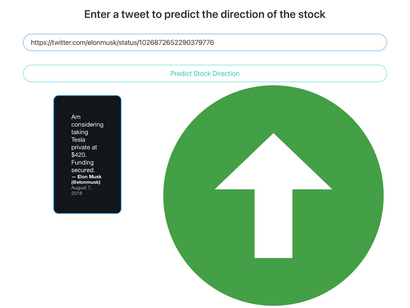
\includegraphics[width=9cm, height=7cm]{2.png}
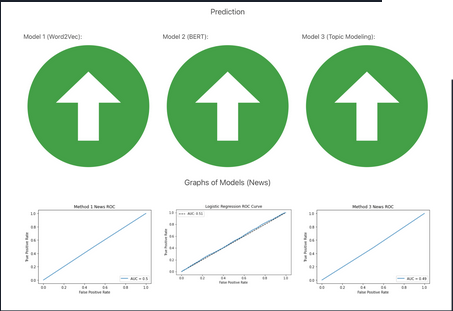
\includegraphics[width=9cm, height=7cm]{1.png}
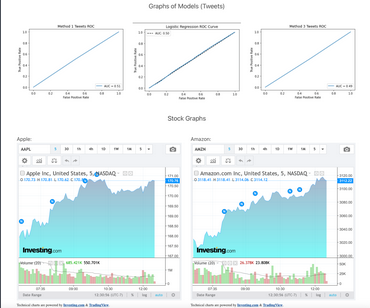
\includegraphics[width=9cm, height=7cm]{3.png}


\section{Task Division and Team Members' Contributions}
\begin{table}[htp]
    \begin{center}
        \begin{tabular}{|l||c|c|} \hline\hline
            Task                                               & Owner         & Deadline  \\ \hline
            Merging news and stock data set                    & Rushil        & 2/18/22   \\
            Data preprocessing, splitting training/testing & Crystal       & 2/25/22   \\
            M1: Word2Vec, sentiment, LR                  & Brian, Joseph & 3/18/22   \\
            M2: BERT, sentiment, LR                & Hadi, Rushil  & 3/18/22   \\
            M3: Topic model, sentiment, Word2Vec, LR     & Crystal       & 3/18/22 \\
            Deliverable: Dashboard                             & Team          & 3/21/22 \\
            Prepare presentation slides                             & Team          & 3/22/22 \\
            Complete Final Report                             & Team          & 4/27/22 \\
            \hline\hline
        \end{tabular}
    \end{center}
\end{table}

\section{Evaluation}
To evaluate the performance of our machine learning models, we split our data sets 80\%-20\% as training data and test data, respectively. We  ran each method on the news data set and the Twitter data set and saw how these two text mediums compare when predicting stock direction. Running all three methods allowed us to compare how different models perform.

The metrics we used are the F1 score and accuracy. The F1 score can be calculated as follows:
\begin{equation*}
 \frac{tp}{tp+\frac{1}{2}(fp+fn)}
\end{equation*}
The accuracy can be calculated as follows:
\begin{equation*}
 \frac{tp + tn}{tp + fp + tn + fn}
\end{equation*}
where $tp$ is the number of true positives, $fn$ is the number of false negatives, $tn$ is the number of true negatives, and $fp$ is the number of false positives. 

Both accuracy and F1 scores are typically used for classification problems. The F1 score is better at taking the distribution of the data into consideration which could be better at measuring performance of data that is heavily imbalanced. On the other hand, accuracy is intuitively easier to understand and performs well when the data is balanced. Since we do not know how the data is distributed yet, we reported both metrics.

The evaluation metrics for the three models used in our project are as follows:




\begin{table}[htp]
    \begin{center}
        \begin{tabular}{|l||c|c|} \hline\hline
            Methods                                               & F1         & Accuracy  \\ \hline
            M1                    & 0.532        & 0.523   \\
            M2 & 0.689       & 0.533   \\
            M3                  & 0.522 & 0.504   \\
            \hline\hline
        \end{tabular}
    \end{center}
\end{table}
where

\begin{itemize}
 \item M1: Word2Vec, Sentiment Analysis, Logistic Regression
 \item M2: BERT, Sentiment Analysis, Logistic Regression
 \item M3: Topic Modeling, Sentiment Analysis, Logistic Regression
\end{itemize}

Overall, the performance of the models did not perform significantly better than a random classifier. The reason behind this could be that more text preprocessing needs to be done or the nature of the data could indicate that a logistic regression model is not the best type of model for this data distribution. Compared to other work done, the models in this project did not perform very different from the other models that were created in previous works. In the previous works that we read about, other groups' models averaged a 50-60\% accuracy which is not far off from our models. 

\section{Conclusions}
Overall, the models performed similarly between the news dataset and the Twitter dataset, even though the jargon between the two differ greatly. Our models performed similarly to previous works done by other individuals and organizations listed above in this report. 

There is plenty of future work that could compliment the work that we have done this semester. For example, we could assign a higher weight to Twitter accounts that have a higher influence determined by metrics such as follower count or industry relevance. This would add another dimension in the feature vector and weigh Tweets from accounts like Elon Musk higher than Tweets from smaller accounts. This could improve the performance of the models that were ran on the Twitter data set. Another extension for this project that we could explore is doing post-model exploratory analysis. We could take a subset of the news headlines that were predicted as a class 0 (decreasing stock price) and look at the similarities of this subset such as the sentiment scores, or perform K-means clustering on the word vectors.

There is still a lot of work to be done in the field of predictive machine learning that can benefit all aspects of life. Working on a stock price predictor could result in a powerful tool for analysts and even the average consumer who likes to participate in the stock market. As algorithms and computer performances advance, perhaps the predictive performance could be greatly improved. 

\begin{thebibliography}{00}
    \bibitem{b1} A. Mittal and A. Goel, “Stock Prediction Using Twitter Sentiment Analysis,” Stanford, 2011. [Online]. Available: https://cs229.stanford.edu/proj2011/GoelMittal-StockMarketPredictionUsingTwitterSentimentAnalysis.pdf. [Accessed: 01-Mar-2022].
    \bibitem{b2} A. O'Shea and C. Davis, “What is the stock market and how does it work?,” NerdWallet, 07-Jan-2022. [Online]. Available: https://www.nerdwallet.com/article/investing/what-is-the-stock-market. [Accessed: 01-Mar-2022].
    \bibitem{b3} C. Nicholson, “A beginner's guide to word2vec and neural word embeddings,” Pathmind, 2020. [Online]. Available: https://wiki.pathmind.com/word2vec. [Accessed: 01-Mar-2022].
    \bibitem{b4} E. Stewart, “Elon Musk's (probably serious) proposal to take Tesla private and the fallout, explained,” Vox, 15-Aug-2018. [Online]. Available: https://www.vox.com/2018/8/15/17692582/elon-musk-tesla-stock-sec-investigation-nasdaq. [Accessed: 01-Mar-2022].
    \bibitem{b5} F. Pascual, “Topic Modeling: An Introduction,” Monkey Learn, 26-Sep-2019. .
    \bibitem{b6} G. Muraski, “How a company's tweets impact its stock prices - temporarily and permanently,” Robert H. Smith School of Business, 29-Nov-2021. [Online]. Available: https://www.rhsmith.umd.edu/research/how-companys-tweets-impact-its-stock-prices-temporarily-and-permanently. [Accessed: 01-Mar-2022].
    \bibitem{b7} J. Brownlee, “Logistic regression for machine learning,” Machine Learning Mastery, 14-Aug-2020. [Online]. Available: https://machinelearningmastery.com/logistic-regression-for-machine-learning/. [Accessed: 01-Mar-2022].
    \bibitem{b8} J. Catlin, “Sentiment Analysis explained,” Lexalytics, 2022. [Online]. Available: https://www.lexalytics.com/technology/sentiment-analysis. [Accessed: 01-Mar-2022].
    \bibitem{b9} J. Si, A. Mukherjee, B. Liu, Q. Li, H. Li, and X. Deng, “Exploiting Topic based Twitter Sentiment for Stock Prediction,” University of Illinois at Chicago, 2013. [Online]. Available: https://www.cs.uic.edu/~liub/publications/ACL-2013-Jianfeng-stock-short.pdf. [Accessed: 01-Mar-2022].
    \bibitem{b10} M. Jermann, Stanford, Palo Alto, California, tech., 2020.
    \bibitem{b11} M. Rizvi, “What is Bert: Bert for text classification,” Analytics Vidhya, 14-Jun-2020. [Online]. Available: https://www.analyticsvidhya.com/blog/2019/09/demystifying-bert-groundbreaking-nlp-framework/. [Accessed: 01-Mar-2022].
    \bibitem{b12} S. R. Varsheni, “Why and how to use BERT for NLP Text Classification,” Analytics Vidhya, 29-Jun-2021. [Online]. Available: https://www.analyticsvidhya.com/blog/2021/06/why-and-how-to-use-bert-for-nlp-text-classification/. [Accessed: 01-Mar-2022].
    \bibitem{b13} T. Naliniprava, "Stock Price Prediction Using Support Vector Machine Approach," International Academic Conference on Management and Economics, 2019. [Online]. Available: https://www.dpublication.com/wp-content/uploads/2019/11/24-ME.pdf. [Accessed: 01-Mar-2022].
    \bibitem{b14} Wei, Feng \& Nguyen, Uyen. (2020). Stock Trend Prediction using Financial Market News and BERT. 325-332. 10.5220/0010172103250332.
\end{thebibliography}
\end{document}
